% !TeX root = progress2.tex

\subsubsection{Progress}
Within the last three weeks, my contributions to the project were mainly confined in testing the quality of the signal in the communication channel and the performing product research for future requirements in the project. The details are discussed below. 
\begin{itemize}
    \item \textbf{Create Eye Diagrams}
    
    Upon observing the BERs against certain SNRs of the communication channel it was suggested by Prof. Killey that we implement an Eye Diagram to observe the quality of the transmitted signal to get a better idea of where the error lies. After doing research into some pre-existing Python packages that could perhaps generate an Eye Diagram for us, I decided it was best if I made the function and plots myself. I went through two models of functions to generate an eye diagram before we settled on our current one.
    \begin{figure}[H]
        \begin{subfigure}[h]{0.53\linewidth}
            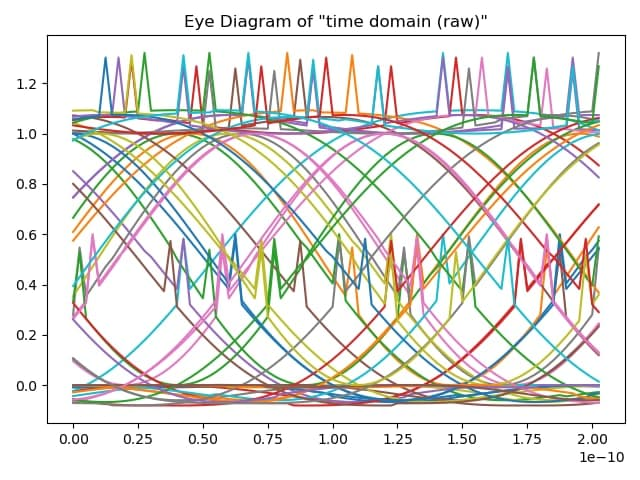
\includegraphics[width=\linewidth]{trial_eye_diagram.jpg}
            \caption{Trial Eye Diagram Model}
        \end{subfigure}
        \begin{subfigure}[h]{0.53\linewidth}
            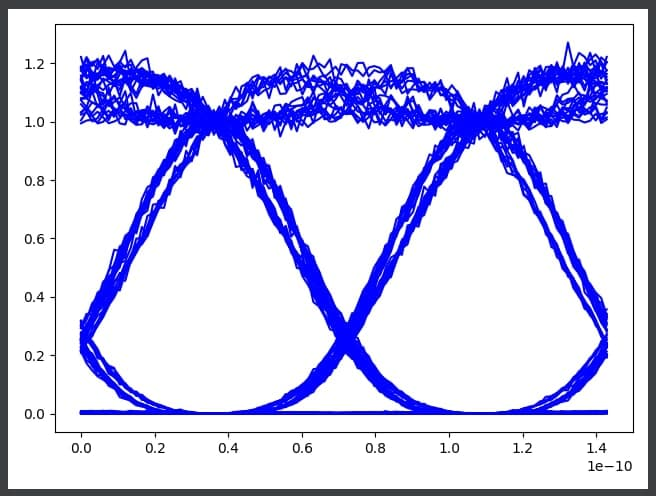
\includegraphics[width=\linewidth]{model_eye_diagram.jpg}
            \caption{Chosen Eye Diagram Model}
        \end{subfigure}
        \caption{Graphs showing the output of the different Eye Diagram Functions}
    \end{figure}
    
    \item \textbf{Research DACs and ADCs}
    
    Currently we are in the simulation stage of our project but after the Christmas holidays we plan to port the model to an FPGA according to our project schedule shown in \textit{\textbf{Table 5.1.1}}. I spent some time researching different DACs and ADCs for the FPGA as suggested by our primary supervisor. After realising that our desired specifications for a DAC/ADC were not feasible (400GSps), I tried lowering the specifications to ~100GSps. This is much more feasible. The majority of my search has been conducted on two companies suggested to me by Prof. Killey: Micram and SocioNext, but I have also looked into Texas Instruments and Fujitsu to see if they have any viable options. At this stage the group are still deciding based on our options. 
\end{itemize}
\subsubsection{Difficulties Encountered}
As I mentioned before, I looked through pre-existing Python packages to see if there was already a function that could build an eye diagram for us and I could just tailor some of the data for that function. As it turned out, none of the packages we had already installed had anything with what I was looking for. I managed to find two packages online but the documentation was scarce and support was little. The results it produces is quite clean and easy to read so I need to spend some time debugging the program. I have not yet been able to do this as we have found another solution that seemed more readily at hand.\newline

In researching product information for DACs and ADCs, I did encounter some difficulty in finding the correct and useful information about the product. I required me to do proper research into our needs and what specifications are generally detailed in each product. Additionally some companies keep this information private and I need to go through UCL as an institution to acquire this product information.